\documentclass[a4paper]{IEEEtran}

\usepackage{graphicx}
\usepackage{hyperref}
\graphicspath{{illustrations/}}

\begin{document}

\setlength{\tabcolsep}{16pt}
\renewcommand{\arraystretch}{1.25}

\begin{center}
  \textbf{\Large{
    Imagely: A cloud environment for online image processing
  }}\\
  \vspace{0.25cm}
  \emph{Authors}: SB~Ramalingam Santhanakrishnan (4740270), \\ K~Kleeberger (???) and B~Jain (???)\\
  ICT Innovation, EEMCS, TU Delft\\
  \emph{Emails}: \{S.B.RamalingamSanthanakrishnan, K.Kleeberger, B.Jain\}@student.tudelft.nl\\
  \vspace{0.2cm}
  \emph{Course Instructors}: DHJ~Epema, A~Iosup and A~Kuzmanovska\\
  PDS Group, EEMCS, TU Delft\\
  \emph{Emails}: \{D.H.J.Epema, A.Iosup, A.Kuzmanovska\}@tudelft.nl\\
  \vspace{0.2cm}
  \emph{Lab Assistant}: BI~Ghit\\
  PDS Group, EEMCS, TU Delft\\
  \emph{Email}: B.I.Ghit@tudelft.nl\\
  \vspace{0.2cm}
  \emph{Teaching Assistant}: A~Parthasarathy\\
  EEMCS, TU Delft\\
  \emph{Email}: A.Parthasarathy@student.tudelft.nl\\
\end{center}

\vspace{0.2cm}

\textbf{
  \emph{Abstract}---\emph{Imagely} is a cloud service for batch image processing, designed for the specific requirements of WantCloud BV. Images are submitted by the end user, which are then processed by the service and the user is notified. It runs on Amazon Web Services (AWS) IaaS barebone compute resources to provide elastic scaling capabilities and its system design adapts the standard master-worker batch processing reference architecture pattern provided by AWS. The scheduler and provisioner are written in NodeJS in reactive style. We run three workloads each on three combinations of VM and scheduling policies with a hundred images. We show that it can achieve a speedup of up to ?? at peak load, compared to the baseline performance of a constant, pre-allocated compute resources. [ADD ONE MAIN RESULT]
}

\section{Introduction}

WantCloud BV is a popular image processing company and are pioneers in converting raw satellite images to standard image formats consumable by users on the web browser. As the company is expanding into other domains and 
adding new customers rapidly, their existing deployment unable to cope up with peak traffic demands and
 maintain service level agreements (SLAs). Thus, WantCloud BV is evaluating an IaaS-based solution that
 can scale with the demand.

The proposed system utilizes Amazon Web Services (AWS)~\cite{aws} IaaS cloud service provider's compute instance, EC2 (Elastic Cloud Compute) for providing on-demand provisioning of compute capacity to process the workloads.
We design a custom provisioner and scheduler using the AWS low-level SDK EC2 API for requesting and releasing instances (VMs).
We also utilize Amazon Machine Images (AMIs) for pre-packaging the application code,
configuration information and the operating system for the instance to save time during its launch. For image processing and conversion, we use the ImageMagick~\cite{imagemagick} program. We wrap ImageMagick with a thin HTTP server written in NodeJS~\cite{nodejs}, which forks ImageMagick as a child process and performs read/write through stdin/stdout pipes, the instances which perform image processing are known as
the workers. For analysis purposes, we restrict the scope of the worker to scaling down, rotating and converting the
image from TIFF~\cite{rfc3302} to JPEG format~\cite{jpeg}.

The system design follows the AWS reference architecture for batch processing~\cite{aws_batch}, except that we have
implemented custom reactive scheduler and provisioner and have placed all the task queues and resource management responsibilities on the master node. The master node accepts the image processing task requests via HTTP and launches multiple worker nodes as per the number of tasks based on the given policy, balances and allocates tasks them and also monitors the progress. It also keeps building a report on completion of each task and launch/release of each instance during its lifetime. The policy targets the provisioner with parameters for minimum and maximum
number of workers to launch and the scaling-up decision threshold.

The test workload is a collection of 100 TIFF images from NASA's publicly available Landsat satellite image repository, file sizes ranging from 40-60 MB. To determine the baseline (current) effort required, we run the workload on a static VM deployment and to analyse the scaling and scheduling capability of the cloud solution, we test the workload with two different threshold policies. The workload itself is varied with three exponential Poisson mean inter-arrival time distributions to simulate realistic request patterns.

In \autoref{application}, additional background information on the application is provided. In \autoref{system_design} we illustrate the design of the system in detail with focus on specific aspects pertaining to
WantCloud's requirements and in \autoref{experiments} we present the experiments conducted along with the
results and analysis. We conclude the report in section~ref{conclusion} with a short discussion on the findings and potential improvements.

\section{Application} \label{application}

The web-based application receives tasks from end-users in JSON format~\cite{rfc7159}, which point to a source image URL and defines a sequence of image manipulation operations such as scaling, rotation and finally file format conversion from TIFF to JPEG. This JSON request is forwarded to an idle worker in the resource pool by the master node. Internally, ImageMagick program is used for processing the image and it is forked by the worker's NodeJS web server. The application is I/O bound during retrieval of the source image and writing the result to AWS S3 storage (the NodeJS web server handles all I/O), CPU and memory intensive when it performs the actual image manipulation and conversion. The worker declares the task as a failure if the above three steps encounter an error or the entire 
task does not complete within 30 seconds (parameterized).

\subsection{Requirements}

In order to replace WantCloud's current system, the following requirements are to be met by the new system.

\begin{itemize}
  \item \emph{Automation}: The system should be automated for creation, provisioning and other activities
  with minimal human intervention.
  \item \emph{Auto-scaling}: The system should be able to detect fluctuations in demand and scale up or down the VM resource pool automatically.
  \item \emph{Load Balancing}: The system should be able to best utilize the available pool of compute resources
  for the workload through allocation policies.
  \item \emph{Reliability}: The system should be able to retry failed tasks, ensure availability through redundancy and recover from unexpected failures.
  \item \emph{Monitoring}: The system should be able to keep track of resource usage and provide information
  on metrics to aid future decisions.
\end{itemize}

\begin{figure}[tbp]
  \centering
    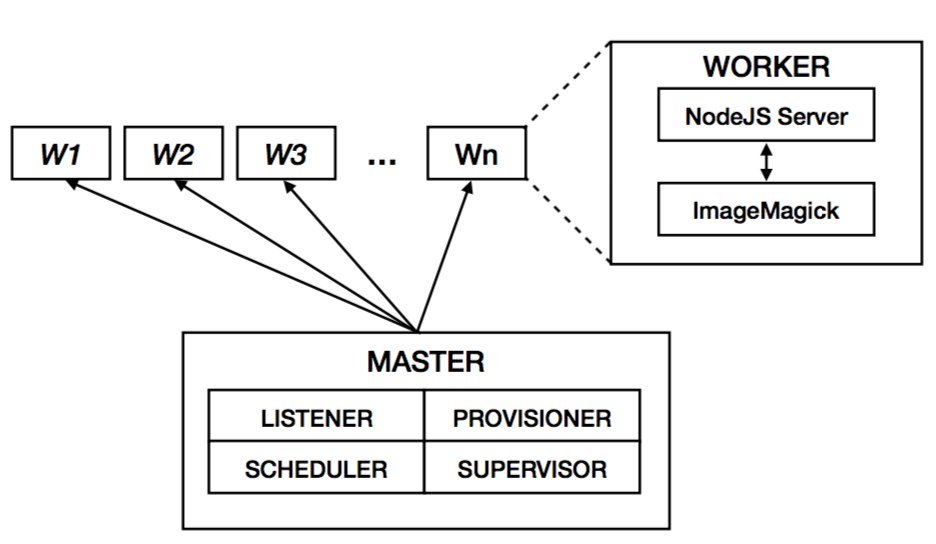
\includegraphics[width=\columnwidth]{system-design.png}
  \caption{Overview of system design.}
  \label{fig:overview_system_design}
\end{figure}

\section{System Design} \label{system_design}

As mentioned in \autoref{application}, the server (master node) accepts the tasks and adds it to the pending task queue. The task is then allocated by the scheduler to an available worker instance at the next scheduling cycle. The workers finish the task and notify the end-user via E-mail about the job completion or failure, the stored location of the result and returns control to the master with usage info.

\subsection{Overview} \label{system_design_overview}

The system, illustrated in \autoref{fig:overview_system_design} consists of the following components, placed in the master node:

 \begin{itemize}
   \item \emph{Listener}: The NodeJS server, which accepts client requests through HTTP, parses it, creates a 
   corresponding internal task representation and adds it to the pending task queue.
   \item \emph{Scheduler}: The scheduler runs periodically and matches tasks in the pending queue to free
   worker instances in the resource pool.
   \item \emph{Provisioner}: The provisioner manages the request and release of worker instances in the resource 
   pool according to the given policy.
   \item \emph{Supervisor}: The supervisor is responsible for bootstrapping the system, monitoring the finished/failed tasks, health of the instances, maintain an audit log of all the tasks and instances to generate a report when requested and finally perform cleanup and release of instances on unexpected shutdown (SIGINT, SIGTERM)
   if possible\footnote{During bootstrap, it queries AWS for any existing workers adds them to the resource pool.}.
 \end{itemize}

\subsection{Resource Management Architecture}
 
\begin{figure}[bp]
  \centering
    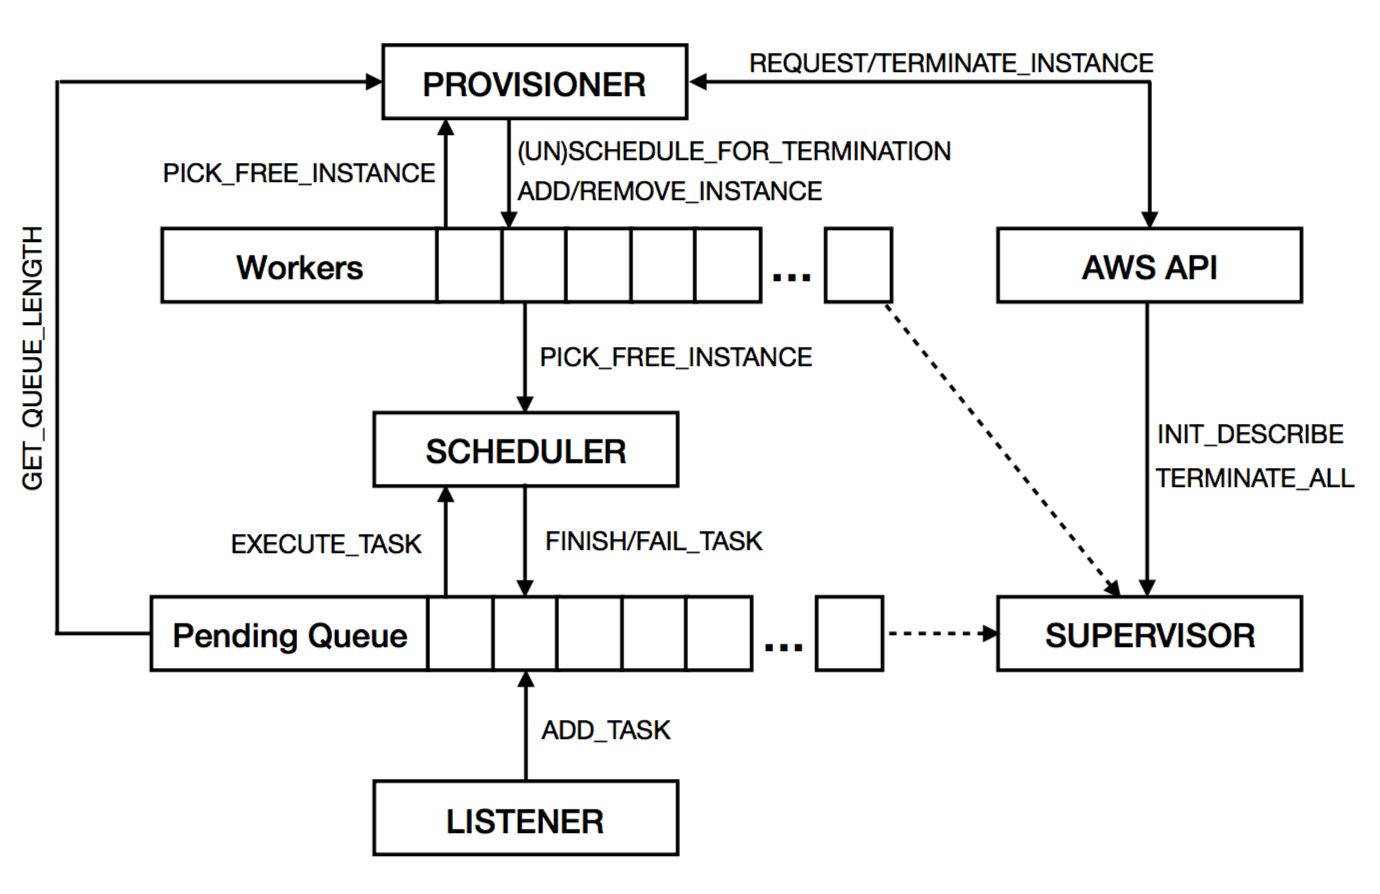
\includegraphics[width=\columnwidth]{resource-management.png}
  \caption{Resource management architecture with message flows.}
  \label{fig:resource_management}
\end{figure}

The components listed in \autoref{system_design_overview} each have their own life cycle and associated events.
Since the we follow the reactive pattern, we illustrate the resource management architecture by tracing the execution
 of a task through the system, handled by the various components across phases listed below and in \autoref{fig:resource_management}.

\begin{enumerate}
  \item \emph{Bootstrap}: This phase marks the start of the system, before the arrival of tasks. The supervisor starts the scheduler, provisioner and the listener and 
  broadcasts a \textsc{Bootstrap} event which the components listen to and perform initial setup activities if any. The supervisor
  also invokes the AWS API with a \textsc{Describe} call to get a list of already started workers if any, this is essential to prevent
  orphaned nodes in case the master restarts for failure recovery.

  \item \emph{Scheduling and Allocation}: The listener listens for incoming tasks from end-users and adds it to the pending queue
  with the \textsc{Add\_Task} event by marking the arrival time. The scheduler is invoked periodically to pick
  tasks from the pending queue, pick free instances from the worker pool, match the two and publish the event \textsc{Execute\_Task}.
  Another part of the scheduler asynchronously listens to \textsc{Execute\_Task}, invokes the worker node, waits till 
  the task is finished/failed and adds it to the pending queue again on failure. The allocation of jobs to workers
  is influenced by three policies -- priority of tasks in the pending queue, criteria of allocation to a worker instance and
  the maximum number of retries for a failed task.

  \item \emph{Provisioning}: The provisioner is also invoked periodically and performs two duties -- pick free instances from the 
  resource pool for termination, request for a new instance based on the given policy. As soon as we request the AWS API
  for a new instance, we repeatedly hit the health check HTTP endpoint of the worker application to determine if its ready
  \footnote{This is possible because AWS allocates a private IP address to the instance as soon as the request is made. In case this 
  is not possible with the cloud provider, we additionally wait for the IP address to be allocated before beginning health checks.}.
  If it is ready before a timeout, it is added to the worker pool else terminated immediately. Note that in regular cases we do not terminate immediately
  instead we first schedule a worker for termination in the future with \textsc{Schedule\_For\_Termination} event, to prevent thrashing.
  A separate part of the scheduler listens to this event, waits for the scheduled time and then releases instance by calling AWS API, however during the
  wait, it also intercepts any calls to request for new instance, cancels the termination schedule and adds the instance back to the pool.
  The policies applied to provisioning are the minimum/maximum number of instances to maintain, queue threshold for scaling
  decisions, and the worker instance type to launch and its placement.

  \item \emph{Termination and Reliability}: During the termination phase, the supervisor shuts down each instance in
  the resource pool with a \textsc{Terminate\_All} call. The reliability of the system is ensured by configuring auto-restart
  of the master process in the host operating system and running it as a daemon process. The supervisor also maintains
  an audit trail of the system, which can be retrieved via an HTTP endpoint for inspection. Since the system is
  single threaded we make sure that the queue and resource pool data structures are maintained in a single
  immutable store and updated only via invocation of events.
  
  To determine the health of the instances, when a task fails the supervisor runs a health check on the instance
  on which the task failed. The failure of the health check leads to immediate termination of the instance.

\end{enumerate}

\subsection{System Policies}

In the system, we have implemented one scheduling policy and one allocation policy listed below.

\begin{enumerate}
  \item \emph{Scheduling}: The scheduler implements the first come, first serve (FCFS) policy.
  It picks the task with the earliest arrival time and maximum retry count for execution on the next available
  worker instance.

  \item \emph{Provisioning}: We implement \textsc{On-Demand Single VM (OD-S)} policy, which allocates 
  one VM per job and releases the VM after job completion plus a wait time (10 seconds in our case). The provisioning
  of new instances is taken when the pending task queue length crosses the given threshold.

  The configurable parameters of the OD-S policy are,
    \begin{itemize}
      \item \emph{min-vms}: The minimum number of VMs the system must have at any point.
      \item \emph{max-vms}: The total number of VMs the system can provision at most.
      \item \emph{threshold}: The pending queue length at which the provisioner is allowed to start a new instance. 
    \end{itemize} 

  \item \emph{Progress Condition}: The system however ensures that a minimum of 1 instance is running in case there are 
  tasks in the pending queue irrespective of the threshold policy. 

  \item \emph{Termination}: When the pending queue length falls below the threshold, the scheduler marks instances to be
  terminated and the provisioner executes the termination after the wait period.
\end{enumerate}

The components of the system intercept events and lookup the central immutable store in order to enforce the policies. 
This flexibility enables us to implement various other policies or combinations of by consuming the entire state of the 
system at any point in time. The system parameters are summarized in \autoref{table:system_params}, * indicates
that we have varied the value according to experiments in the following section.

\begin{table}[tbp]
  \centering
  \begin{tabular}{|r|r|}
    \hline
     MAX\_RETRIES & 5 \\
     MIN\_VMS & * \\
     MAX\_VMS & * \\
     THRESHOLD & * \\
     MAX\_RETRIES & 5 \\
     SCHEDULER\_INTERVAL & 5s \\
     TASK\_TIMEOUT & 25s \\
     PROVISIONER\_INTERVAL & 5s \\
     HEALTH\_CHECK\_INTERVAL & 1s \\
     INSTANCE\_READY\_TIMEOUT & 60s \\
     TERMINATION\_WAIT\_TIME & 10s \\
     \hline
  \end{tabular}
  \vspace{0.25cm}
  \caption{System parameters and values in implementation.}
  \label{table:system_params}
\end{table}


% \section{Experimental Results} \label{experiments}

% We perform all the experiments on the AWS cloud platform, restricted to a single region North Virgina (US-East-1) with default availability zone and the default virtual private cloud settings.
% A custom security group is used for exposing ports 8000 (master server), 3000 (worker server) and 3001 (worker health check) for inbound TCP (HTTP) traffic.

% \subsection{Experimental Setup}

%  We have extended our custom AMI from the base public Ubuntu image provided by Amazon (id = ami-cd0f5cb6). Workloads have been created from the publicly available image files of NASA's 
%  Landsat-I satellite (x images, total y MB). The workloads are varied by arrival time distribution in order to evaluate the provisioning policies. Each job in the workload requests the given image
%  to be scaled down to 25\% of the original size, rotated by 90 degrees clockwise and converted to
%   JPEG. We generate and send the workloads to the system using custom scripts. The instance type 
%   we use for both master and worker is m3.medium (general purpose compute, vcpu=1 and memory=3.75Gb).

% \subsection{Experiments}

% The goal of our experiments is to measure various workload execution and VM metrics on running the
%  static policy and the dynamic policies and analyse the results to understand the inherent
%  tradeoffs in the elasticity of cloud environments. \footnote{TODO: for each experiment, list
%   \emph{Charged-time}, \emph{Charged-cost} and \emph{Service metrics of the experiment}
% }
 
% \subsubsection{Baseline}

% We determine the makespan of the three workloads on a single unit (SU) instance to analyze 
% the relative speedups and cost-tradeoff in later experiments.

% \subsubsection{Overheads}

% We identify a major overhead in the system due to the time taken for a newly launched VM to 
% reach the ready state. To measure this, we repeatedly request, wait till ready and release a 
% single VM instance for 25 times.

% \subsubsection{Provisioning Policy}

% We exercise three workload variants, linear, bursty and poisson across the three allocation policies,

% \begin{itemize}
%   \item \textsc{CONSTANT-5}, constantly 5 VMs.
%   \item \textsc{OD-S-0}, threshold set to 0, 2 to 20 VMs.
%   \item \textsc{OD-S-5}, threshold set to 5, 2 to 20 VMs.
% \end{itemize}

% \subsubsection{Utilization}

% Utilization is the ratio of the total time spent by the workers in executing the jobs to the
% total lifetime (including boot time) of the workers, described by equation~\autoref{eq:utilization}.

% \begin{equation} \label{eq:utilization}
%   Utilization = \frac{\sum T_{execution}}{\sum T_{lifetime}}
% \end{equation}

% \subsubsection{Speedup vs Cost Tradeoff}

% We summarize the results obtained from the previous experiments and compare the cost and speedup
% of the policies on the workloads.

\section{Conclusion} \label{conclusion}

\bibliographystyle{unsrt}
\bibliography{large-lab}

\section*{Appendix A: Time Sheets}

\begin{table}[htbp]
  \centering
  \caption{Time spent on the project per activity.}
  \begin{tabular}{| l | r | r |}
    \hline
    Activity & Time (hours) \\
    \hline
    Total & \\
    Think & \\
    Dev & \\
    XP & \\
    Analysis & \\
    Write & \\
    Wasted & \\
    \hline
  \end{tabular}
\end{table}

\begin{table}[htbp]
  \centering
  \caption{Time spent per experiment.}
  \begin{tabular}{| l | r | r | r |}
    \hline
    & \multicolumn{3}{| c |}{Time (hours)} \\
    \hline
    & Dev & Setup & Total \\
    \hline
    Baseline & & & \\
    Overheads & & & \\
    Provisioning & & & \\
    Utilization & & & \\
    Speedup & & & \\
    \hline
  \end{tabular}
\end{table}

\end{document}